\documentclass[a4paper,12pt]{assignment}

%----------------------------------------------------------------------------------------
%	NAME AND CLASS INPUT SECTION
%----------------------------------------------------------------------------------------

\newcommand{\hmwkTitle}{\texttt{molSimplify} version 1.0} % Assignment title
\newcommand{\hmwkDate}{April,\ 2016} % Delivery date
\newcommand{\hmwkAuthor}{E. Ioannidis} % Your name
\newcommand{\hmwkProblem}{} % Problem
\usepackage[numbers]{natbib}
\usepackage{bibentry}
\usepackage[most]{tcolorbox}
\definecolor{block-gray}{gray}{0.6}
\newtcolorbox{term}{colback=block-gray,grow to right by=-10mm,grow to left by=-10mm,
boxrule=0pt,boxsep=0pt,breakable}
\usepackage{listings}



\nobibliography* 
\begin{document}
\maketitle

\tableofcontents

\clearpage

\section{General information}

molSimplify is an open source utility that incorporates geometric manipulation routines necessary for the generation of transition metal complexes, automated setup and completion of electronic structure calculations, post-processing and data analysis. The software generates a variety of coordination complexes with any number of metals coordinated by ligands in a single or multidentate (chelating) fashion. The code can both build the coordination complex starting from a single metal atom or work to functionalize a more complex structure (e.g. a porphyrin or other metal-ligand complex) by including additional ligands or replacing existing ones. molSimplify builds intermolecular complexes for evaluating binding interactions and generating candidate reactants and intermediates for catalyst reaction mechanism screening and also supports interaction with chemical databases. Furthermore, it provides a Graphical User Interface (GUI) and is thus accessible to a wider audience since it does not require a lot of prior computational chemistry experience.

\subsection{Obtaining molSimplify}
The binaries, source code and useful documentation can be obtained online by visiting: \url{http://molsimplify.mit.edu}. 


\subsection{Citing molSimplify}

Any published work that utilizes molSimplify shall include the following reference:\\ 

\bibentry{Ioannidis2016}
\newpage{}
\subsection{License}
\subsubsection{molSimplify}
The software is distributed free of charge under the GPL license: \\  \\
\textit{Copyright 2016 Kulik Lab @ MIT\\ \\
    molSimplify is free software: you can redistribute it and/or modify it under the terms of the GNU General Public License as published by the Free Software Foundation, either version 3 of the License, or (at your option) any later version. molSimplify is distributed in the hope that it will be useful,  but WITHOUT ANY WARRANTY; without even the implied warranty of MERCHANTABILITY or FITNESS FOR A PARTICULAR PURPOSE.\\    See the GNU General Public License for more details.     You should have received a copy of the GNU General Public License 
    along with molSimplify. If not, see http://www.gnu.org/licenses/.
}
\subsubsection{Pybrain}
molSimplify makes use of the open-source Pybrain library (\url{http://pybrain.org/pages/home}) for neural network implementation. This work is not endorsed by Pybrain. Pybrain is licensed under the BSD licence:\\

\textit{Copyright 2008, IDSIA and TU M\"{u}nchen (TUM)
All rights reserved.}
\\
\textit{Redistribution and use in source and binary forms, with or without
modification, are permitted provided that the following conditions are met:}
\begin{itemize}
   \item \textit{Redistributions of source code must retain the above copyright
      notice, this list of conditions and the following disclaimer.}
    \item \textit{Redistributions in binary form must reproduce the above copyright
      notice, this list of conditions and the following disclaimer in the
      documentation and/or other materials provided with the distribution.}
    \item \textit{Neither the name of the associated institutions nor the
      names of its contributors may be used to endorse or promote products
      derived from this software without specific prior written permission.}
\end{itemize}

\textit{THIS SOFTWARE IS PROVIDED BY THE DEVELOPERS ''AS IS'' AND ANY
EXPRESS OR IMPLIED WARRANTIES, INCLUDING, BUT NOT LIMITED TO, THE IMPLIED
WARRANTIES OF MERCHANTABILITY AND FITNESS FOR A PARTICULAR PURPOSE ARE
DISCLAIMED. IN NO EVENT SHALL THE DEVELOPERS OR THEIR INSTITUTIONS BE LIABLE FOR ANY
DIRECT, INDIRECT, INCIDENTAL, SPECIAL, EXEMPLARY, OR CONSEQUENTIAL DAMAGES
(INCLUDING, BUT NOT LIMITED TO, PROCUREMENT OF SUBSTITUTE GOODS OR SERVICES;
LOSS OF USE, DATA, OR PROFITS; OR BUSINESS INTERRUPTION) HOWEVER CAUSED AND
ON ANY THEORY OF LIABILITY, WHETHER IN CONTRACT, STRICT LIABILITY, OR TORT
(INCLUDING NEGLIGENCE OR OTHERWISE) ARISING IN ANY WAY OUT OF THE USE OF THIS
SOFTWARE, EVEN IF ADVISED OF THE POSSIBILITY OF SUCH DAMAGE}


\subsection{Acknowledgments}
This software was developed by Efthymios I. Ioannidis, JP Janet, Terry Z. H. Gani  and Heather J. Kulik at the Massachusetts Institute of Technology. The authors would like to especially thank Terry Z. H. Gani for thoroughly testing the code and providing valuable feedback.


\section{Installation}
\subsection{System requirements}
The binaries and the source code have been tested on 64-bit Ubuntu 14.14 and on 64-bit OSX 10.10.7 and are expected to work on any newer system equipped with Python 2.7 or greater. No particular memory requirements or processor capabilities are needed. 

\subsection{Conda Package}
Conda (\url{http://conda.pydata.org/docs/}) is a free, multi-platform and multi-language package and environment manager. Using Conda, it is possible to easily obtain molSimplify and all the environmental dependencies in one step. This is the recommended method for end users to acquire molSimplify. In order to acquire molSimplify using Conda, follow these directions:

\begin{enumerate}
\item Ensure you have an up-to-date version of Conda installed. Binary installers are available for all platforms from \url{https://www.continuum.io/downloads} - we recommend using Anaconda (as opposed to Miniconda).
\item Ensure that you have an up-to-date version of the Anaconda Cloud Client by running
\begin{lstlisting}[language=bash]
  $ conda list -n anaconda-client
\end{lstlisting} 
If the package is not found,  you need to install it (we recommend running this command as SU on Linux systems):
\begin{lstlisting}[language=bash]
  $ sudo conda install anaconda-client
\end{lstlisting} 

\item Now you are ready to install molSimplify by running:
\begin{lstlisting}[language=bash]
  $ conda install -c hjkgroup molSimplify
\end{lstlisting} 
Here, '-c' means that the files will come from the Anaconda Cloud, and hjkgroup is our repository there. Don't forget the capital S! This single command will bring openbabel with python bindings with it, if they are missing. 
\item If you want to use the GUI (graphical user interface), you'll need PyQt5, which you can get (if you don't have it) with 
\begin{lstlisting}[language=bash]
  $ conda install -c dsdale24 pyqt5
\end{lstlisting} 
\item Now you are ready to go! Launch molSimplify from the terminal using:
\begin{lstlisting}[language=bash]
  $ molsimplify 
\end{lstlisting} 
You can add any arguments here in the normal manner, for example:
\begin{lstlisting}[language=bash]
  $ molsimplify -core Fe -lig water -ligocc
\end{lstlisting} 
would generate a 6-coordinated iron-hexaaqua complex.
\end{enumerate}


While Conda remains our recommended method, other installation options exist:

\subsection{From source}
In order to install molSimplify from source it is necessary to install openbabel with its Python bindings (pybel) and numpy. Furthermore, additional software is required in order to use the Graphical User Interface (GUI).

\subsubsection{Linux}

For Linux Ubuntu, the only requirements are a working version of Openbabel with the Python bindings (pybel) and Numpy installed. To install numpy, you can follow the online instructions or use pip install numpy. We suggest installing pybel from source using the following procedure:
\begin{enumerate}
\item   wget \url{https://sourceforge.net/projects/openbabel/files/openbabel/2.3.2/openbabel-2.3.2.tar.gz}
\item  tar -xvf openbabel-2.3.2.tar.gz 
\item mkdir build ; cd build
\item cmake .. -DPYTHON\_BINDINGS=ON
\item sudo make
\item sudo make install
\end{enumerate}.

In order to enable the GUI, the library PyQt5 with its dependencies needs to be installed first. In order to do that we suggest the following procedure:
\begin{enumerate}
\item Download and install Qt5 from source (\url{developer.qt.nokia.com/}). 
\item Install SIP(\url{http://pyqt.sourceforge.net/Docs/sip4/installation.html}) from source. If Python.h is missing use \texttt{sudo apt-get install python-dev} . 
\item Install PyQt5 from source (\url{http://downloads.sourceforge.net/project/pyqt/PyQt5/}).
\end{enumerate}

Once you have installed PyQt5, open an interactive Python terminal window and check whether \begin{lstlisting}[language=python] import PyQt5 \end{lstlisting} works. \\

Once you have installed Pybel (and optionally PyQt5), you proceed with the installation. Obtain the source files from \url{https://github.com/hjkgrp/molSimplify/tree/JP}. Uncompress the zipped directory, and then navigate to top level directory in the unzipped structure. The program can then be installed with
\begin{lstlisting}[language=bash]
  $ sudo python setup.py install
\end{lstlisting} 
The code can then be used from the command line as described in the Conda section.

\subsubsection{Mac OSX}

In order to run molSimplify from source, we need to install pybel first. We suggest using \texttt{brew} as explained in section \ref{osxbin} or compiling from source. Then install imagemagick (see section \ref{osxbin}). In order to use the GUI, PyQt5 and its dependencies need to be installed as well. The easiest way is to use the following procedure:

\begin{enumerate}
\item Install Qt5 with: \texttt{sudo brew install qt5}
\item Install SIP with: \texttt{sudo brew install sip}
\item Install PyQt5 from source (\url{http://downloads.sourceforge.net/project/pyqt/PyQt5/}) with option -\hspace{0.02cm}-sip-incdir=/usr/local/include
\end{enumerate}

Once the correct dependenices are installed, you can follow the same setup instructions as in the Linux case.

\subsection{Binaries}

Binaries of the program have been compiled for both Ubuntu Linux and OSX. The installation of the binaries depends on the platform and analytical instructions are given below.

\subsubsection{Linux}\label{linbin}

For Linux Ubuntu, the only requirement is a working version of Openbabel with the Python bindings (pybel) installed. We suggest installing pybel from source using the following procedure:
\begin{enumerate}
\item   wget \url{https://sourceforge.net/projects/openbabel/files/openbabel/2.3.2/openbabel-2.3.2.tar.gz}
\item  tar -xvf openbabel-2.3.2.tar.gz 
\item mkdir build ; cd build
\item cmake .. -DPYTHON\_BINDINGS=ON
\item sudo make
\item sudo make install
\end{enumerate}

Alternatively pybel can be installed using the standard ubuntu package manager with \texttt{apt-get install python-openbabel}.

In both cases, once the installation is complete, open an interactive Python terminal and make sure that \texttt{import openbabel} and \texttt{import pybel} work before running molSimplify. 

With pybel installed, the user can download the binary and the supporting files and run the program. The program will guide the user in order to set up a configuration file that is stored under \texttt{/home/user/.molSimplify} in the user's home directory and contains a line that specifies the installation directory (top directory) of the program where all the supporting files are located. The line has the format \texttt{INSTALLDIR=path}. The binary can be moved anywhere, however if the top directory of molSimplify is moved the \texttt{.molSimplify} file will have to be manually updated. The configuration file contains also the paths for files used in database search and post processing analysis (see section \ref{dbpp}).

\subsubsection{Mac OSX}\label{osxbin}

For OSX, a package installer has been created that automatically installs the required software for running the molSimplify app. The user can open the \texttt{molSimplify.pkg} installer, follow the instructions and get molSimplify installed.

If the package installer fails, the user can manually install the required packages and then download a copy of the molSimplify app. Two packages are required in order to run the molSimplify app, pybel and imagemagick. The easiest way to install both is to use the \texttt{brew} package manager and issue the following commands on a terminal window:
\begin{enumerate}
\item sudo brew install open-babel -\hspace{0.02cm}-with-python
\item sudo brew install imagemagick
\end{enumerate}

With pybel installed, the user can download the app, place it under /Applications/molSimplify.app and run the program.

If \texttt{brew} is not installed, install it by running \texttt{/usr/bin/ruby -e "\$(curl -fsSL https://raw.githubusercontent.com/Homebrew/install/master/install)"} in a terminal window.



\subsection{Installed files}

With both the binaries or the source code a set of additional files are stored that are required by molSimplify. If you use molSimplify with the molSimplify.app (OSX) these files are stored under /Applications/molSimplify.app/Contents/Resources/, otherwise they are in the installation directory of molSimplify as indicated in the \texttt{.molSimplify} file in the home directory. These additional files include the following:
\begin{itemize}
\item icons: Folder containing the icons used in the GUI.
\item Data: Folder containing the available coordinations/geometries and Metal-Ligand bond length database.
\item Cores: Folder containing the local saved cores.
\item Ligands: Folder containing the local saved ligands.
\item Bind: Folder containing the local saved extra molecules.
\end{itemize}

You can manually update the contents of these folders, however it is recommended to use the modules included in the GUI in order to update them. \\

In the Conda version, package resource management is handled by Conda and Python, and you don't need to worry about them.

\subsection{Databases \& Post-processing}\label{dbpp}

\subsubsection{Chemical database setup}


The program is able to interact with external chemical databases such as ChEMBL. These databases are essentially sdf files that contain information about molecules. In order to link these databases to molSimplify the user needs first of all to download the database sdf file. 

Once the file is downloaded, we recommend using Openbabel's fast search index generation by issuing  \texttt{babel DBfile.sdf -ofs}. Openbabel will then create a .fs file that can be used for fast screening and will substantially accelerate the database search. Note that OpenBabel can handle sdf files smaller than 4GB, so you may have to break larger files before fast indexing them. 

All the sdf and fs files should be placed inside a common directory. Then by clicking on the search DB window on the GUI, a prompt will ask you to specify that directory. Once you specify the directory containing your sdf and fs files, molSimplify will automatically detect them and the database search will be ready to use. Alternatively the user can specify the path by modifying the \texttt{.molSimplify} file in the home directory and adding a line with \texttt{CHEMDBDIR=path}. 

A short list of available chemical databases is:
\begin{itemize}
\item ChEMBL \url{https://www.ebi.ac.uk/chembl/}
\item eMolecules \url{https://www.emolecules.com/}
\item ChEBI \url{http://www.ebi.ac.uk/chebi/}
\item Zinc \url{http://zinc.docking.org/}
\item PubChem \url{http://pubchem.ncbi.nlm.nih.gov/}
\end{itemize}

\subsubsection{Multiwfn setup}

Many of the features included in the post processing module of molSimplify depend on the external program Multiwfn. The user needs to manually install Multiwfn from \url{https://multiwfn.codeplex.com/} and then specify the installation directory by clicking the post processing option in the GUI and then following the prompt instructions.  Alternatively the user can specify the path to the Multiwfn executable by modifying the \texttt{.molSimplify} file in the home directory and adding a line with \texttt{MULTIWFN=path}.




\newpage

\section{GUI overview}

Using the main window of the Graphical User Interface (GUI-Figure\ref{GUIov}), the user is able to access most of the functionality of molSimplify. On the left of the main window, the input options for building and customizing structures can be specified. On the bottom left, clicking the corresponding buttons the user can list the available ligands, cores and extra molecules as well as add new molecules to the local database. In the middle, there are options for randomly generating structures and general options for building complexes. Finally on the right, the user can specify additional molecules for studying intermolecular interactions, parameters for generating quantum chemistry input files and queuing system jobscripts.

\begin{figure}[htb!]
\centering
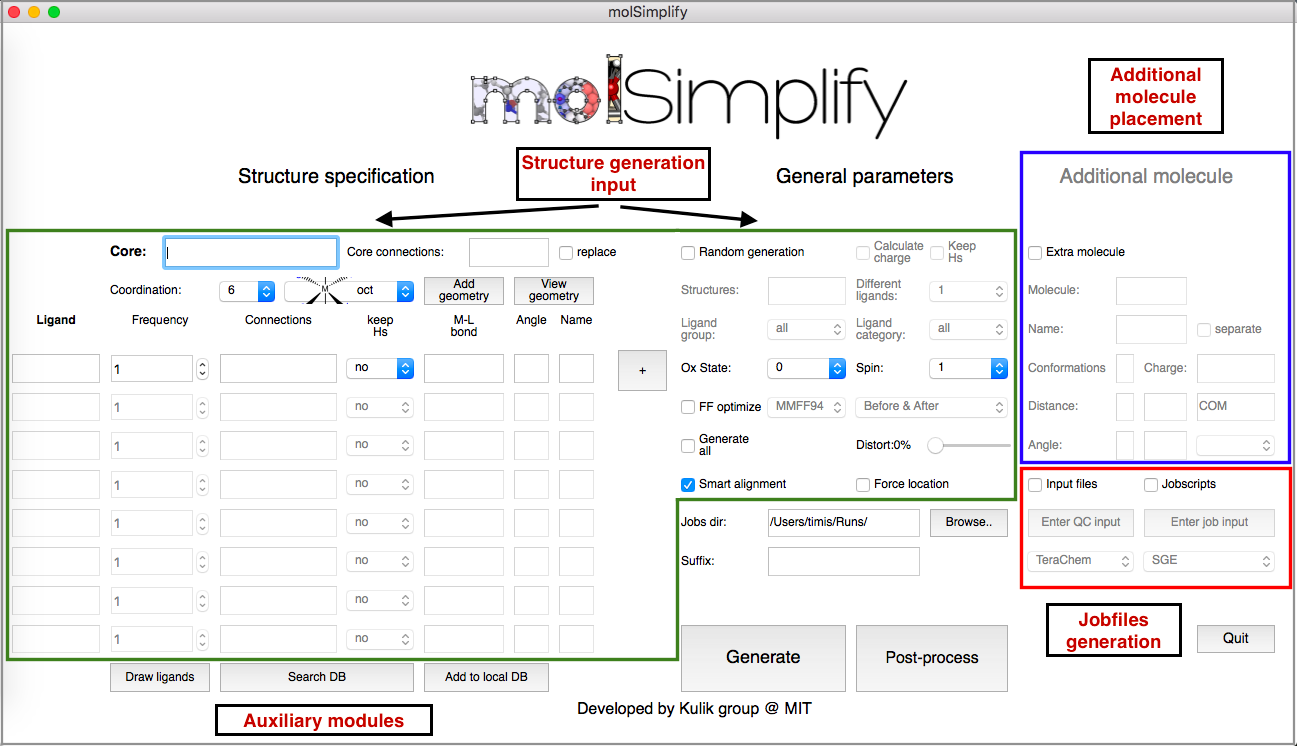
\includegraphics[width=\textwidth]{./Figures/fig0.png}
\caption{The main window of the GUI where the structure generation is coordinated.}
\label{GUIov}
\end{figure}


In all cases where the GUI is used, an input file is generated and stored in the jobs directory under the names \texttt{geninput.inp} for the structure generation module, \texttt{dbinput.inp} for the database search module and \texttt{postproc.inp} for the post-processing module. The program can be used without the gui by running from the command line and specifying the input file using the \texttt{-i} flag (e.g. molSimplify -i geninput.inp). The software supports command line arguments as well. An input file can be generated from the GUI using the \textit{Save as} button and existing input files can be loaded back to the GUI using the \textit{Load} button.

The program also generates a log file named \texttt{molSimplify.log} in the jobs  directory where the input options and additional information is being printed for debugging and logging.

\section{Structure generation module}
The main function of molSimplify is building new structures or editing existing ones. In this part of the user guide, several examples for building structures are included. 

\subsection{Building simple structures}\label{simpgen}

Building a simple symmetric metal coordination complex in molSimplify requires minimal input by the user. As an example, we are going to build an octahedral, 6-coordinate complex with a single cobalt metal in the middle and 6 ammonia ligands coordinated around (Figure \ref{genl} left). The corresponding input parameters on the GUI and the generated input file are shown below.

\begin{figure}[htb!]
\centering
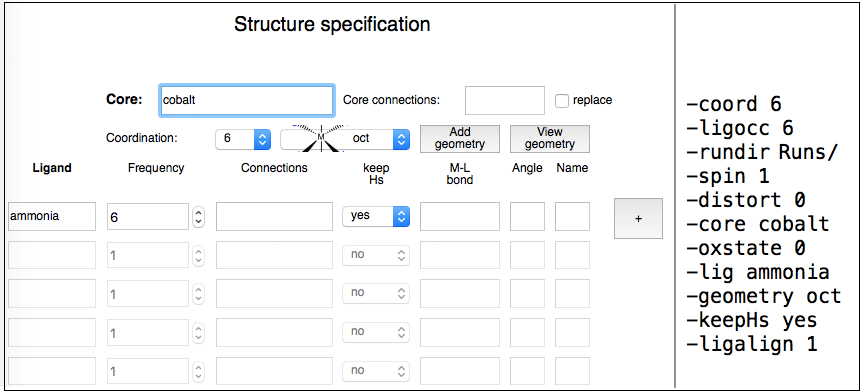
\includegraphics[width=\textwidth]{./Figures/fig1.png}
\caption{Input parameters for building a simple symmetric octahedral complex using either the GUI or an input file.}
\label{GUIov}
\end{figure}

On the top left of the GUI, the user needs to specify first the core structure. This core structure can be either a predefined atom or molecule from the local database or a new one in SMILES format or a file path to an xyz or mol file. For example, the following are valid cores for molSimplify: \texttt{iron, [Fe], $\sim$/iron.xyz}. Multiple cores can be also specified separating them with comma or whitespace. The program will then loop and generate one structure for each specified core. Multiple cores are also supported in other features such as the random generation (see section \ref{rgen}).

 Next, the coordination is specified by selecting first the coordination number on the metal (6 in this example) and then a corresponding geometry (octahedral here). New geometries can be added using the appropriate option and the current geometry can be viewed by clicking the \texttt{View geometry} button.

Once the core is specified, the user needs to specify the ligands that are going to be attached to the core. In this example, we only use one ligand, namely ammonia. A ligand can be either a predefined atom or molecule, a SMILES string or a path to an xyz/mol file (for example: \texttt{ammonia, N, $\sim$/NH3.xyz} are all valid options). Once the ligand is specified under the \texttt{Ligand} field, the frequency or number of copies of that ligand is specified. In our symmetric ligand we are just going to use 6 ammonia copies (specified on the \texttt{Frequency} field). The field \texttt{Connections} contains the indices of the atoms on the ligand that are going to be connected to the metal and for predefined ligands (such as ammonia), it's not required. Because the program by default strips one Hydrogen from the connection atom of the ligand (to allow the bond formation with the metal), we need to specify that we want to keep all Hydrogens in ammonia by selecting \texttt{yes} in the \texttt{keep Hs} field, otherwise we would end up with NH$_2$ instead. Next, in the \texttt{M-L bond} field, the user can overwrite the default value and specify a custom Metal-Ligand (in this case cobalt-nitrogen) bond length in Angstroms. The software contains a database with trained Metal-Ligand bond lengths collected from various DFT simulations and it uses this information if available. In case the Metal-Ligand pair is not present in the database, the program searches for a similar pair or uses the sum of the covalent-radii to approximate the bond. Next, the user can distort the specified geometry by selecting a pair of angles (see section \ref{cangle}). Finally, if the user requests a ligand using a file path or a SMILES string, a name for that ligand can be specified (not required for predefined ligands).

The same options can be specified using an input file (automatically generated if using the GUI). Along with the options specified in Core/Ligand fields, some additional options are included by default in the input file. In this case the keyword \texttt{-coord} specifies the coordination number, \texttt{-ligocc} the frequency of the ligands, \texttt{-rundir} the directory where the structure files will be placed, \texttt{-spin} the spin multiplicity of the system (by default it's 1), \texttt{-distort} the percentage of random distortion of the geometry (by default it's 0), \texttt{-core} specifies the core of the structure, \texttt{-oxstate} specifies the oxidation state of the metal (default is 0), \texttt{-lig} the ligands included in the structure, \texttt{-geometry} the geometry of the complex, \texttt{-keepHs} whether to keep the Hydrogens on the ligand's connection atom (default no) and \texttt{-ligalign} is a flag that forces a specific order when the complex is being built (see section \ref{force}).

Once the program finishes it generates an xyz file with the coordinates of the desired structure (Figure \ref{genl}, left).


\begin{figure}[htb!]
\centering
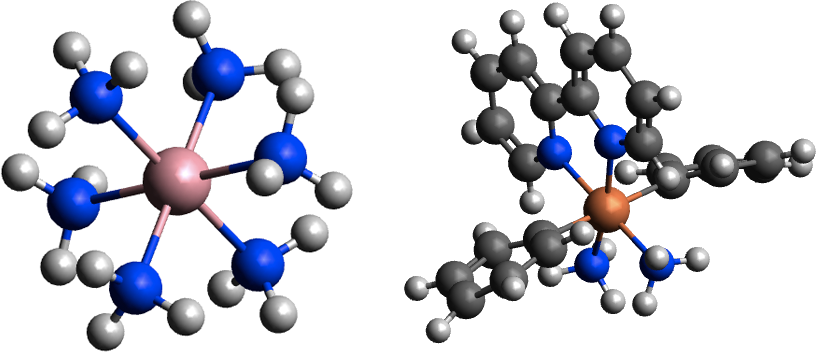
\includegraphics[scale=0.5]{./Figures/figen.png}
\caption{Left:A six-coordinated octahedral structure with a cobalt center and 6 ammonia ligands around. Right: A six-coordinated octahedral structure with an iron center, 2 benzenes, 2 ammonias, and 1 bipyridine around.}
\label{genl}
\end{figure}

\subsection{Building more complicated structures}\label{compgen}

In case of asymmetric structures, more ligands need to be specified in the input. In this example we are going to generate again an octahedral, 6-coordinate structure, this time with an iron center and 3 different ligands, namely ammonia, benzene and bipyridine (Figure \ref{genl}, right). The GUI options and the corresponding input file are shown in Figure \ref{multilig}.

\begin{figure}[htb!]
\centering
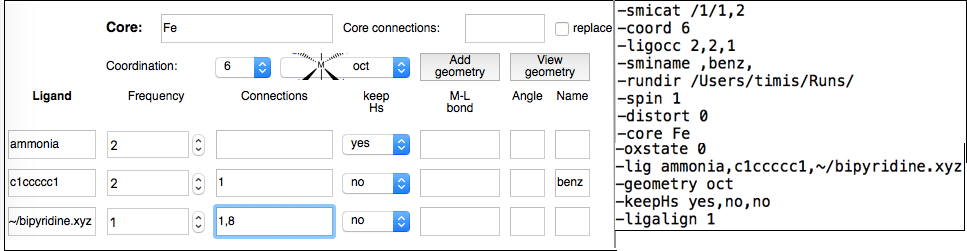
\includegraphics[width=\textwidth]{./Figures/fig2a.png}
\caption{Input parameters for building more complicated structures.}
\label{multilig}
\end{figure}

Once the core and coordination are specified, the options for the 3 different ligands have to be included. Initially, we select ammonia from the list of predefine ligands as in the previous example, however here we only want 2 copies of the ligand, thus we select 2 in the \texttt{Frequency} field. Next, we specify 2 copies of a benzene ligand using its corresponding SMILES string $c1ccccc1$ and selecting 2 in the \texttt{Frequency} field. Because this ligand is not predefined we also need to specify the index of the atom that is going to be connected to the metal (a carbon atom). The user can visualize the ligand with its atom labels in a molecular viewer such as Avogadro, or use the \texttt{View ligands} option on the bottom left of the GUI to locate the correct connection atom index (Figure \ref{drawlig}). When the \texttt{View ligands} option is selected, the program will draw a 2D representation of the ligands with their atomic labels and also generate a png image inside the running directory. In this case atom 1 corresponds to a carbon atom on the ring that is going to get a Hydrogen stripped before it gets connected to the metal (option \texttt{no} in the \texttt{keep Hs} field). We use the default values for M-L bond length and do not distort the octahedral geometry (empty \texttt{M-L bond} and \texttt{Angle} fields) and name this ligand \texttt{benz} using the \texttt{Name} field. Similarly, we specify the last ligand which in this case is bipyridine, defined using an input file located at \texttt{$\sim$/bipyridine.xyz}. Because this ligand is chelating and connects to the metal center with 2 connection atoms (bidentate), we need to specify 2 indices in the \texttt{Connections} field. If we visualize the ligand, we can see that the 2 nitrogens that are coordinating the metal center have the atomic labels 1 and 8 (Figure \ref{drawlig}).


\begin{figure}[htb!]
\centering
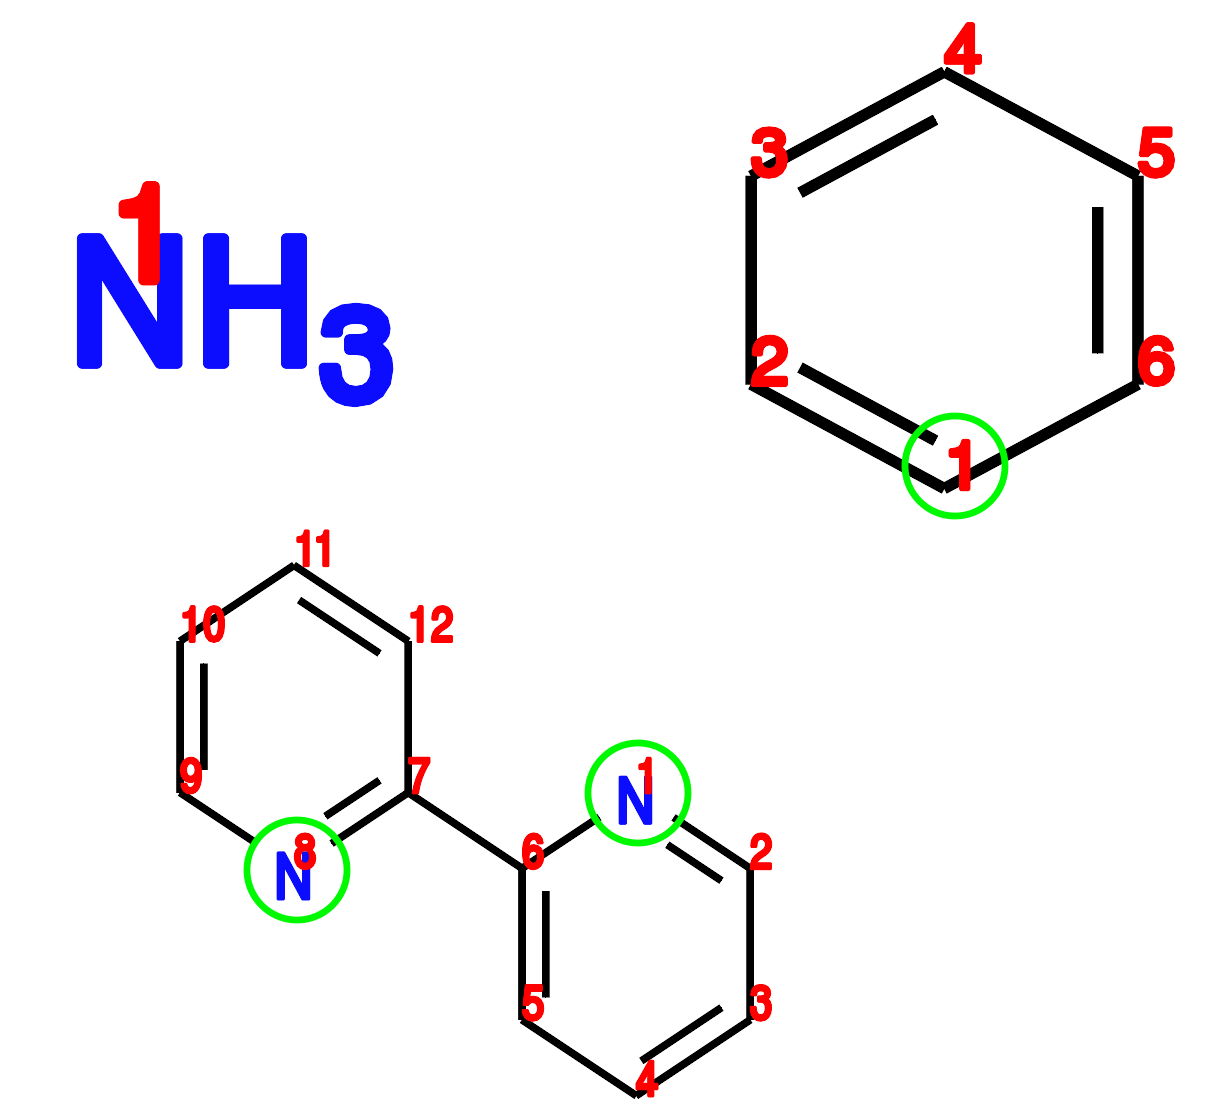
\includegraphics[scale=0.15]{./Figures/fig2b.png}
\caption{2D representation of ligands with their corresponding atomic labels. Highlighted are the connection atoms for each particular ligand that need to be specified in the input.}
\label{drawlig}
\end{figure}

In the corresponding input file, the connection atoms are specified with the \texttt{-smicat} keyword and are separated with '/' for each ligand (predefined ligands just need an empty value).


\subsection{Force field optimization}\label{sffopt}

In order to improve the quality of the generated structures, molSimplify has several options for relaxing them using force fields. The program supports 4 different force fields (default and recommended is MMFF94) and 3 different optimization options. Using the \texttt{Before} option, the several ligands included in the generation are force field optimized in isolation, before they are attached to the metal core. Using the \texttt{After} option, the ligands are force field optimized along with the metal core after they have been attached. In this option the whole structure is being optimized in the end as well, however the metal center is ignored and the connection atoms of the ligands held fixed during the optimization. Finally using the \texttt{Before \& After} option, both \texttt{Before} and \texttt{After} optimizations are performed. In order to enable force field optimization, the user needs to select the corresponding option on the GUI or use the \texttt{-ff} keyword in the input file (Figure \ref{ffopt}). Note that in some cases (such as very small ligands) FF optimization is not necessary or can result in worse structures. Therefore, ligands can be blacklisted by removing the force field optimization option during addition to to the database.

\begin{figure}[htb!]
\centering
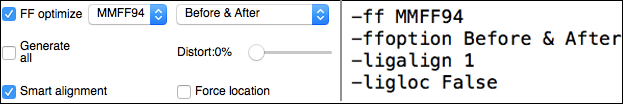
\includegraphics[width=\textwidth]{./Figures/fig3.png}
\caption{Force field optimization input parameters in the GUI and in the input file.}
\label{ffopt}
\end{figure}

By selecting the generate all checkbox or specifying the corresponding keyword in the input file (\texttt{-genall True}), the program will automatically generate 4 xyz files. One with trained Metal-Ligand (ML) bond lengths and FF optimization, one with trained ML bond lengths and without FF optimization, one with simple covalent radii guess for the ML bond lengths and with FF optimization and one with covalent radii guess for the ML bond lengths and without FF optimization. This feature is particularly important in cases where the user doesn't know a priori if FF improves the predicted structure and if the trained ML bond length is a good estimate of the true bond length.



\subsection{Smart alignment \& Force order}\label{force}

In the previous examples, the options \texttt{Smart alignment} and \texttt{Force location} were first mentioned. The first option which is enabled in the input file with the keyword \texttt{-ligalign True} tells molSimplify to use a smart alignment algorithm. This means, that the order that the ligands will be attached to the metal will be shuffled according to their denticities and size so that the best possible structure is obtained (default is True).

The \texttt{Force location} feature can be used in order to generate complexes with desired stereochemical properties. By default, molSimplify will attach ligands to the best possible positions on the coordination template and not necessary in the order specified by the user. If the user wants to attach ligands to specific points in space, the force location option needs to be enabled. For example, let's say we have a pentagonal bipyramidal structure as shown in Figure \ref{ord}, where we want to attach an ammonia ligand in position 1, a bipyridine ligand in positions 2 and 3, 2 carbonyls in positions 4,5 and 2 water molecules in the axial positions 6,7. In order to do that, we specify the ligands in the correct order (fist ammonia, then bipyridine, then carbonyl and then water) and select the force location option to get the desired location. Force location and smart alignment are 2 independent options, the first one specifying the location of each ligand and the second one the order that the ligands will be attached.

\begin{figure}[htb!]
\centering
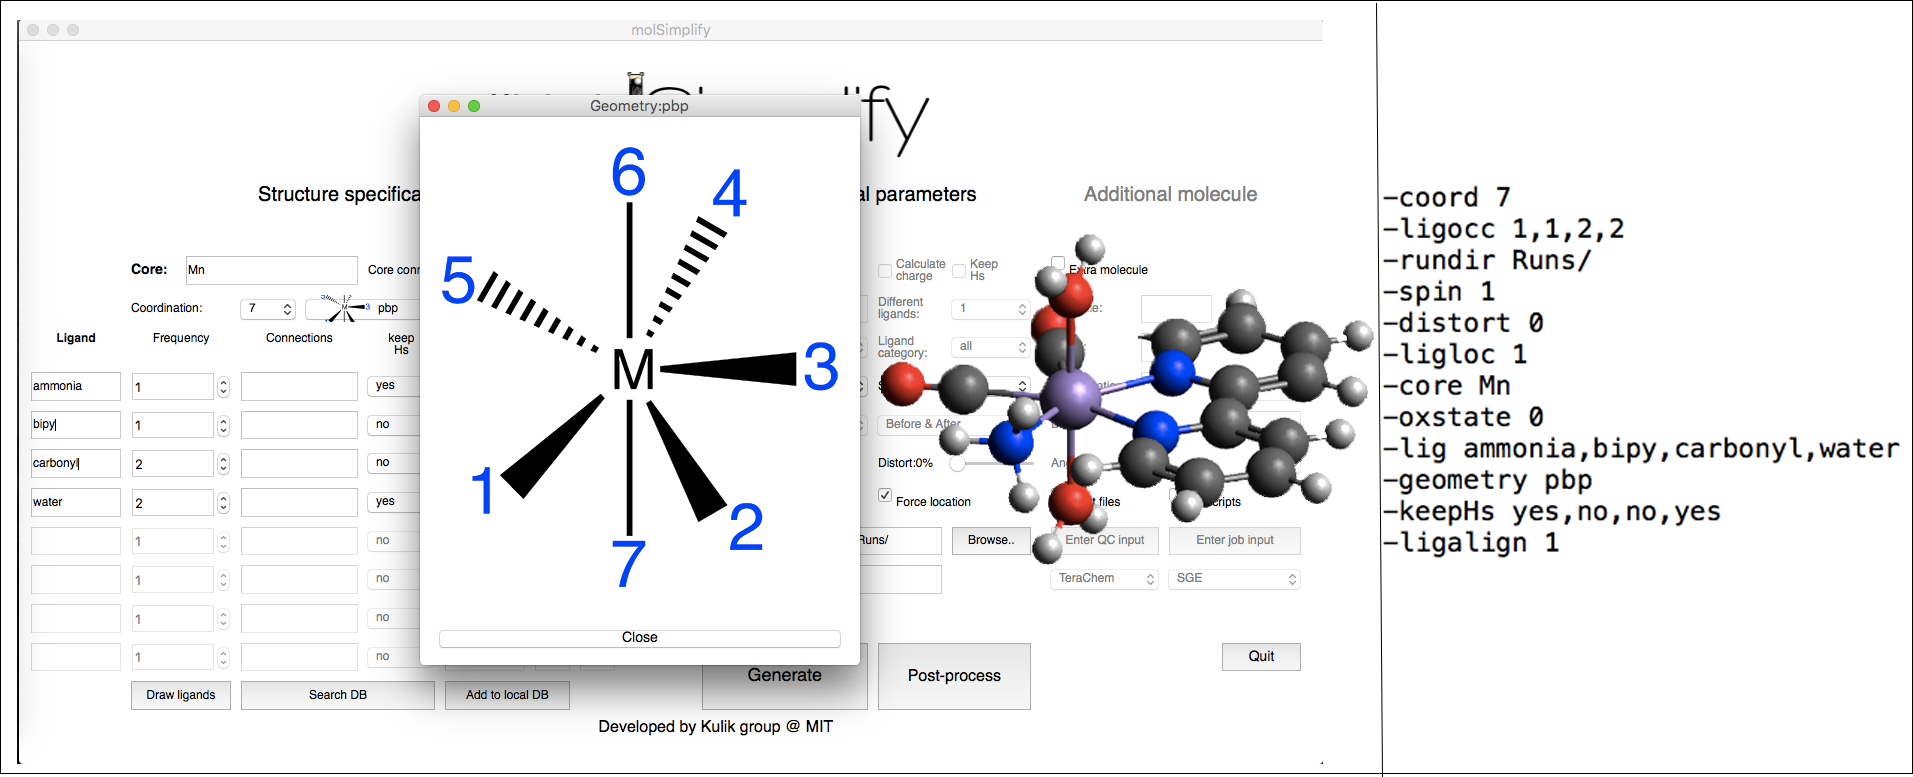
\includegraphics[width=\textwidth]{./Figures/fig12.png}
\caption{Input options for custom core ligand replacement.}
\label{ord}
\end{figure}

Additionally, if the user wants for example to have 2 ammonia ligands at specific points, 2 separate entries are needed in the ligands table, both with ammonia as the ligand but in different rows that correspond to the desired connection points on the geometry template.

\subsection{Custom angles}\label{cangle}

The user has fine control of the predefined geometries. The default connection points for the ligands can be distorted according to the needs of the specific application. For each ligand two distortion angles can be specified in the corresponding \texttt{Angle} field on the ligand table. The first one is a polar angle $\theta$ (0-360$^o$) and the second one an azimuthal angle $\phi$ (0-180$^o$) and correspond to a spherical coordinate system centered at the corresponding connection point. As an example we are going to generate an octahedral complex with 3 different ligands, carbonyl, cyanide and ammonia, with two of them corresponding to distorted sites on the octahedral complex (Figure \ref{lang1}). The two angles are separated using '/' on the corresponding field and the default value is 0.0/0.0 (no distortion). In the input file, the custom angles are specified with the keyword \texttt{-pangles}.

\begin{figure}[htb!]
\centering
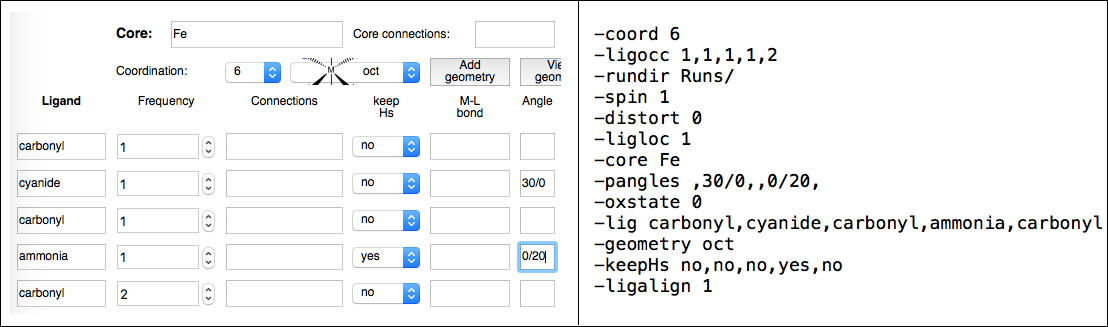
\includegraphics[width=\textwidth]{./Figures/fig13a.png}
\caption{Input options for distorting the default geometry by custom angles.}
\label{lang1}
\end{figure}

The cyanide ligand will have a 30$^o$ distortion along the polar direction which can be specified using the value $30/0$ in the corresponding \texttt{Angle} field on the table. In Figure \ref{lang2}, top right, we can see that cyanide is bent by 30$^o$. Similarly, the ammonia ligand that is connected to point 4 will be distorted by an azimuthal angle of 20$^o$ as can be seen in Figure \ref{lang2}, bottom right.

\begin{figure}[htb!]
\centering
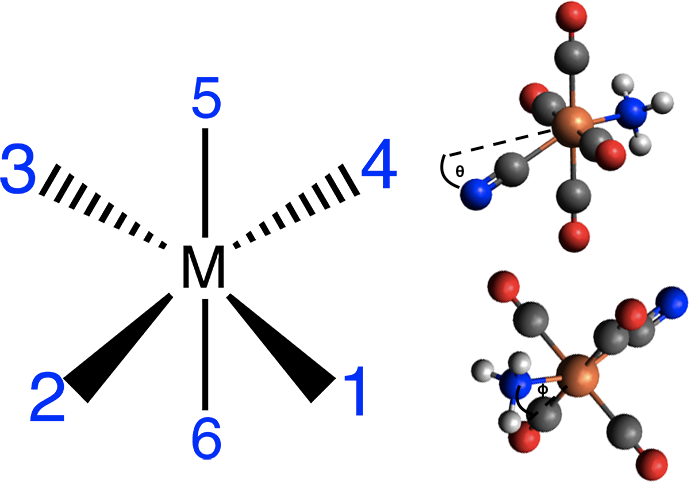
\includegraphics[width=0.6\textwidth]{./Figures/fig13b.png}
\caption{Two examples of distorted coordination geometries. On the left is the default octahedral geometry, on the top right the cyanide ligand is distorted by a polar angle of 30$^o$, while on the bottom right an ammonia ligand is distorted by an azimuthal angle of 20$^o$.}
\label{lang2}
\end{figure}

\subsection{Building custom structures}

The program is able to generate structures using non-standard cores. If the user specifies a core that is not a single metal center, then the coordination and geometry specified will be ignored and a custom structure will be built instead. Any structure can be used as core, on which additional ligands will be attached. For example, we are going to generate a complex using an iron porphyrin as our core structure and functionalize it with imidazole rings in 4 points (Figure \ref{custom0}).  

\begin{figure}[htb!]
\centering
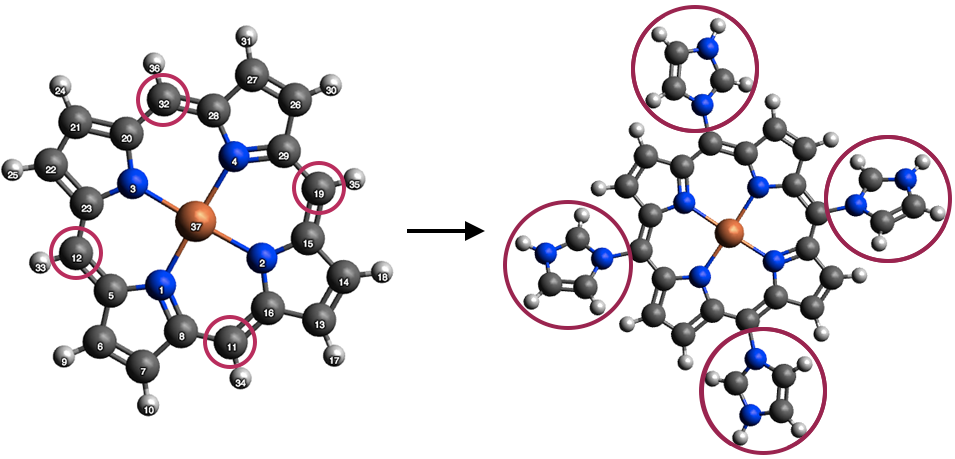
\includegraphics[width=\textwidth]{./Figures/fig4a.png}
\caption{Custom core functionalization.}
\label{custom0}
\end{figure}

First, the user needs to specify the iron porphyrin as the core which in this case is done through a mol file. Then the user needs to specify the indices of the atoms on the core where the ligands are going to be attached. In this case, we select 4 carbon atoms with indices 11,12,19 and 32 and specify them in the \texttt{Core connections} field. Then, we need to specify again the ligands we are going to use (in this case 4 copies of the standard imidazole molecule). This input is specified on the top left of the GUI (Figure \ref{custom1}).

\begin{figure}[htb!]
\centering
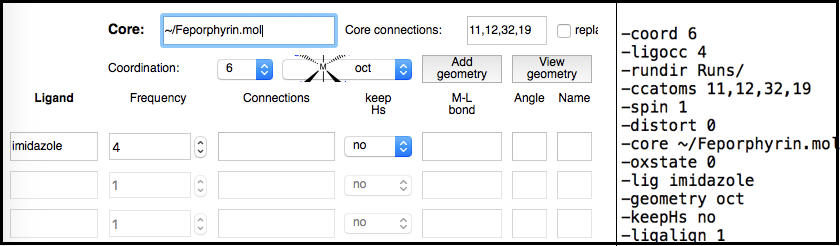
\includegraphics[width=\textwidth]{./Figures/fig4b.png}
\caption{Input options for custom core functionalization.}
\label{custom1}
\end{figure}

The same input can be specified in an input file using the corresponding keywords. The keyword \texttt{core} specifies the custom core, but this time we also need the keyword \texttt{ccatoms} to specify the atoms on the core that are going to be connected with the ligands. The rest of the input is similar to the simple coordination complexes case. Once the generation is complete, a new porphyrin structure will be generated with 4 imidazole rings (Figure \ref{custom0}).



\subsection{Replacing existing ligands}

Another feature that molSimplify offers is editing existing structures by replacing existing ligands with new ones. In order to enable this feature the user needs to enable it by clicking the \texttt{replace} checkbox on the GUI or specify the \texttt{replig} option in the input file.

As an example we are going to take the functionalized iron porphyrin that we generated in the previous example and replace 2 of the imidazole rings with benzene (Figure \ref{rep0}). 

\begin{figure}[htb!]
\centering
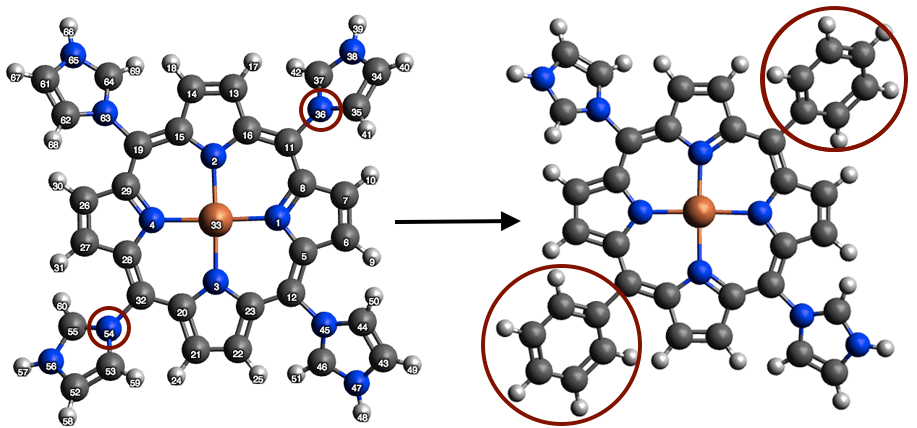
\includegraphics[width=\textwidth]{./Figures/fig5a.png}
\caption{Custom core ligand replacement.}
\label{rep0}
\end{figure}

Initially, we need to specify the functionalized porphyrin as our new core structure using the xyz file that we generated earlier. In this case though, as connection atoms the user needs to specify the connection atoms on the \textbf{ligands} that are going to be replaced and are connected to the metal and not the atoms on the old core that are going to receive the ligands. In the case of imidazole the connections are the nitrogen atoms that are bonded with the carbons on the porphyrin, namely atoms 36 and 54. Then, the new ligands that are going to replace the existing ones are specified in the ligand table. These options are specified again on the GUI or the input file directly (Figure \ref{rep1}).

\begin{figure}[htb!]
\centering
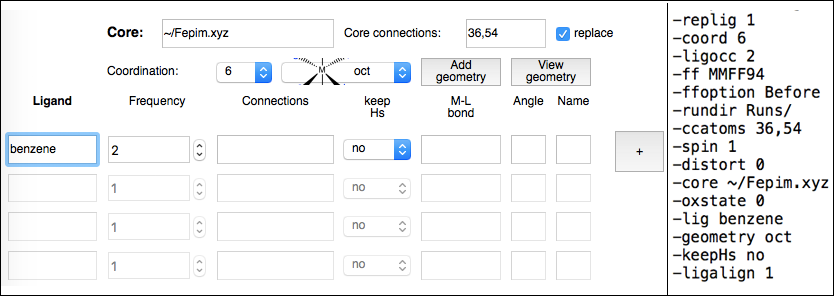
\includegraphics[width=\textwidth]{./Figures/fig5b.png}
\caption{Input options for custom core ligand replacement.}
\label{rep1}
\end{figure}

The program loops over the specified connection points, removes the old ligands and replaces them with the new ones for a new final structure (Figure \ref{rep0}). Note that the force field optimization options described earlier (see section \ref{sffopt}) can be used in custom core building or editing as well.


\subsection{Additional molecule placement}

In order to study intermolecular interactions, molSimplify is able to build supramolecular complexes by placing additional molecules around the initially generated structure, a feature denoted as \texttt{Additional} or \texttt{Extra molecule} placement.

\begin{figure}[htb!]
\centering
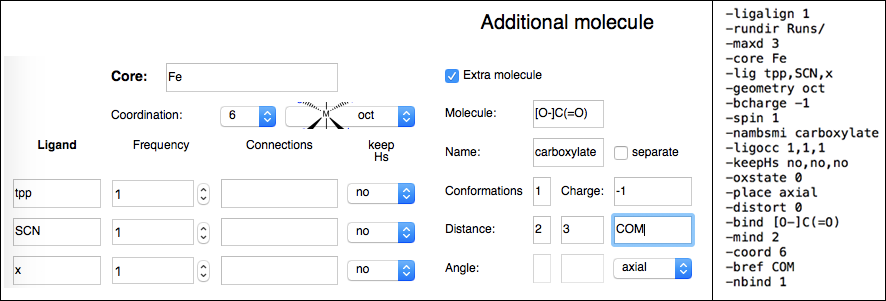
\includegraphics[width=\textwidth]{./Figures/fig6.png}
\caption{Input parameters for additional molecule placement.}
\label{ex1a}
\end{figure}

As an example we are going to place a simple carboxylate (formate) around an octahedral porphyrin structure in order to calculate the binding energy of the carboxylate on the core structure (Figures \ref{ex1b}-\ref{ex1c}). Initially the user specifies the base structure, namely a tetraphenylporphyrin (tpp) with an iron center, a thiocyanate (SCN) ligand on the first axial position and an empty site denoted as the \texttt{x} ligand on the other axial position. We include an empty site here so that the additional molecule can be placed close to that point and then bind on that site.

Once the base structure is specified according to sections \ref{simpgen}-\ref{compgen}, we need to tell the program where to place the additional molecule and what kind of molecule that is. This is done on the \texttt{Additional molecule} block on the GUI (top right) by enabling the \texttt{Extra molecule} input. In the \texttt{Molecule} field we can again specify a predefined molecule from the local database, a SMILES string or a file path to an xyz or mol file. The corresponding keyword in the input file is \texttt{-bind}. Next we select a name for the complex (carboxylate in this case, keyword \texttt{-nambsmi} in the input file). The flag \texttt{separate} can be used to separate the two complexes in the QChem input file for running super-position error corrections for example. Next we select how many copies of the system we want in the \texttt{Conformations} field (keyword \texttt{-nbind}). Because by default the program uses random placement of the extra molecule we might want to explore different ways of binding and by specifying multiple conformations, different placements of the extra molecule will be generated. Then we can specify the charge of the complex in the corresponding field (keyword \texttt{-bcharge} in the input file). 

\begin{figure}[htb!]
\centering
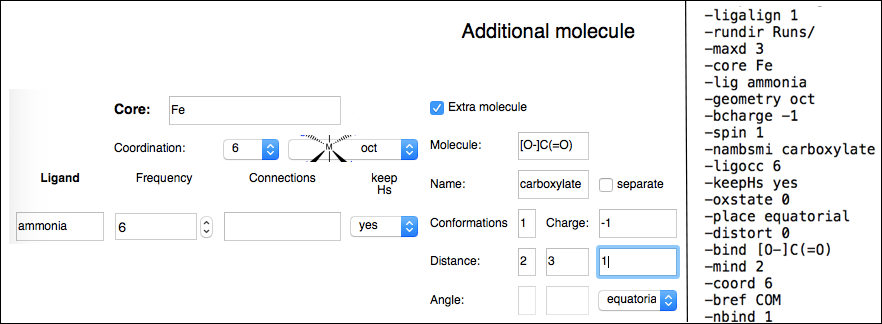
\includegraphics[width=\textwidth]{./Figures/fig7a.png}
\caption{Input parameters for additional molecule placement.}
\label{ex1b}
\end{figure}
In the next line we can specify the distance of the additional complex relative to the base structure. The first field corresponds to the minimum distance in Angstroms while the second to the maximum distance (keywords \texttt{-mind} and \texttt{-maxd} respectively). The last field (COM in this case, denoting Center of Mass) tells the program the reference point on the additional for the distance calculation (keyword \texttt{-bref}). In this case the center of mass of the extra molecule will be placed between 2 and 3 Angstroms from the base structure. Other options are atomic indices or element symbols (e.g. specifying \texttt{C} here would place the extra molecule in such a way that the carbon on the formate would be between 2 and 3 Angstroms from the base structure). In the last row of the input, we can specify the orientation of the placement by selecting either a set of angles (azimuthal angle (0-180$^o$) and polar angle (0-360$^o$) with respect to the base structure (keywords \texttt{-bphi} and \texttt{-btheta} respectively) or by selecting axial or equatorial placement (keyword \texttt{-place}). In this case, because we want the carboxylate to be placed on top of the porphyrin, the axial option was selected. The final placement is shown in Figure \ref{ex1c} (left).

As an additional example, we can place the same formate molecule on the equatorial position of a symmetric iron-ammonia complex by changing the corresponding flag in the \texttt{Angle} row (Figure \ref{ex1b}).

\begin{figure}[htb!]
\centering
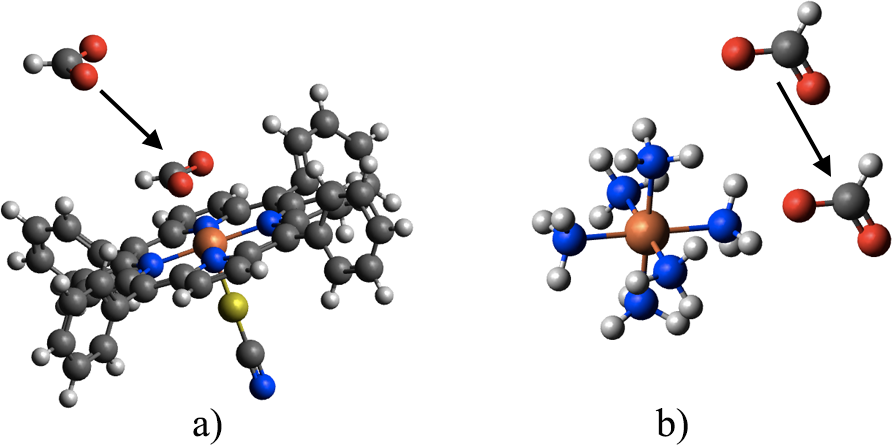
\includegraphics[width=\textwidth]{./Figures/fig7b.png}
\caption{Examples of extra molecule placement.}
\label{ex1c}
\end{figure}

When the additional molecule option is selected, a minimum of 3 xyz files will be generated, one with the base structure only, one with the additional molecule only and one with the combined structure.


\section{Random generation module} \label{rgen}

One of the most useful features of molSimplify for novel structure generation is the random generation module. By enabling this feature, the user is able to perform a constrained random generation of a big number of complexes. In this module, the user specifies a limited number of input parameters and the program randomly selects the rest. As an example, we will generate a set of 10 different square pyramidal structures with chromium core, 4 ammonia ligands on the planar sites and 10 random ligands on the axial position (Figure \ref{ran1a}).

\begin{figure}[htb!]
\centering
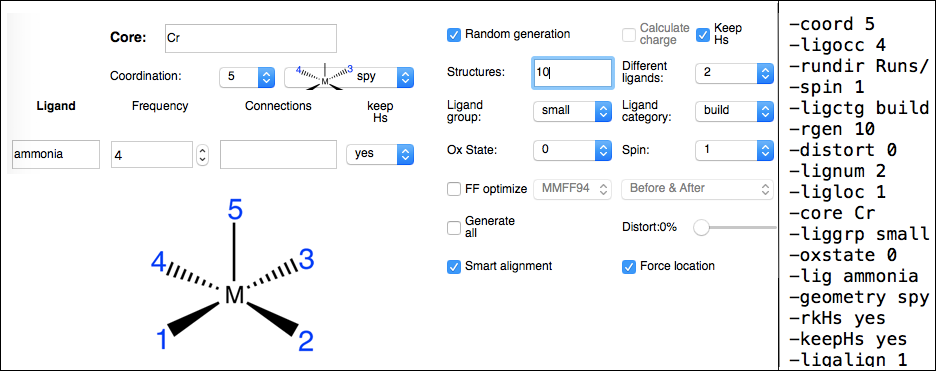
\includegraphics[width=\textwidth]{./Figures/fig8a.png}
\caption{Input options for custom core ligand replacement.}
\label{ran1a}
\end{figure}

In order to do that, we first specify the constraints, namely the chromium core and the 4 ammonia ligands following the same procedure as for normal structure generation. Next, in the random generation block we specify the number of different structures that we want in the \texttt{Structures} field (keyword \texttt{-rgen} in the input file) and then the number of different ligands that we want in the final structure (field \texttt{Different ligands} or keyword \texttt{-lignum} in the input file). In this case we already have ammonia as the first ligand and we want one additional one, therefore the total number of different ligands is only 2. Next we can limit the search for random ligands by selecting ligands from specific groups or categories using the corresponding options on the GUI or the keywords \texttt{-liggrp} and \texttt{-ligctg} respectively. Finally, we need to turn the force location option on to ensure that the random ligand will be placed on the axial position, otherwise the program might try to change the ligand locations. Note that we have selected to keep Hydrogens on the random ligands as well (keyword \texttt{-rkHs} in the input file).


\begin{figure}[htb!]
\centering
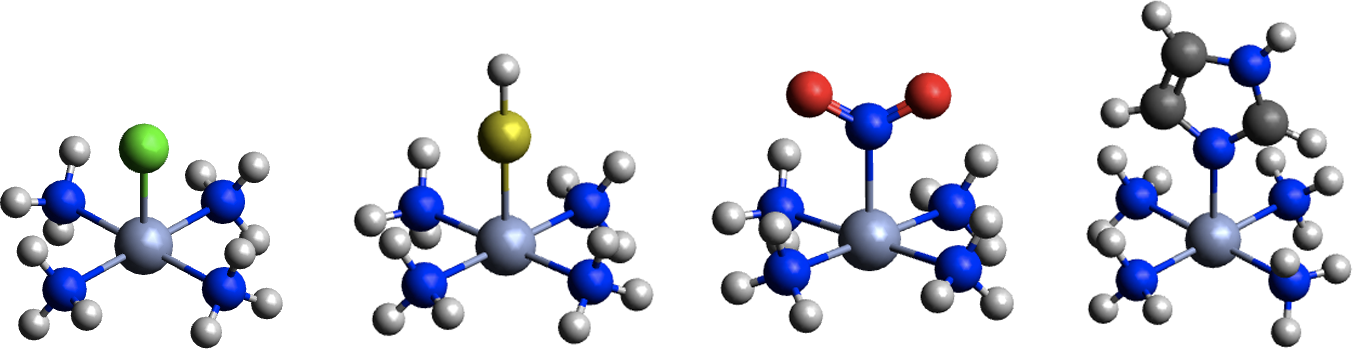
\includegraphics[width=\textwidth]{./Figures/fig8b.png}
\caption{Input options for constrained random generation.}
\label{ran1b}
\end{figure}

Once the structure generation is complete, a set of xyz files will be generated each corresponding to a different structure (Figure \ref{ran1b}) that conforms with the constraints imposed by the user.

\begin{figure}[htb!]
\centering
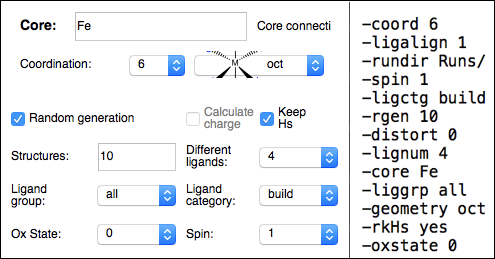
\includegraphics[width=\textwidth]{./Figures/fig9a.png}
\caption{Example structures obtained from the random structure generation.}
\label{ran2a}
\end{figure}

As an additional example, we will generate a set of random octahedral structures with iron center. In this case, we don't specify any ligands, thus all of them will be randomly generated. We just specify the core of the structure (iron), the number of random structures that we want and the number of different ligands that we want (4 different ligands here).

\begin{figure}[htb!]
\centering
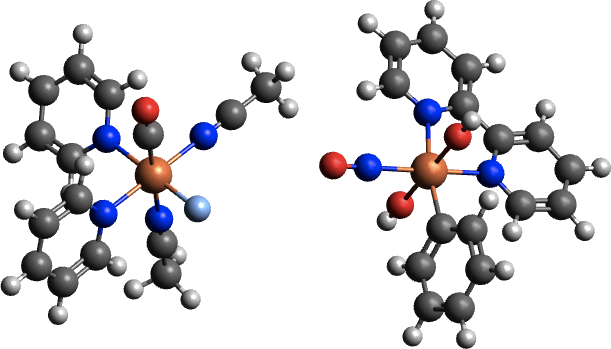
\includegraphics[width=0.75\textwidth]{./Figures/fig9b.png}
\caption{Example structures obtained from the random structure generation.}
\label{ran2b}
\end{figure}

Two example output structures are shown in Figure \ref{ran2b}, each with 4 different ligands. The first one has a chlorine, a carbonyl, two imidazole rings and two acetonitrile ligands. The second one has a bipyridine, a benzene ring, 2 hydroxyls and a nitroso ion. 


\section{Input files \& jobscripts}
In addition to generating the structures, molSimplify is able to generate input files for Quantum Chemistry (QC) calculations and jobscripts for submitting jobs in supercomputer queues. Currently, molSimplify supports 3 QC programs: TeraChem, GAMESS-US, QChem and 2 queuing systems, SGE and SLURM.


\subsection{Input file generation}

In order to generate QC input files, the corresponding checkbox should be selected on the GUI or the keyword \texttt{-qccode} specified in the input file. In this example, we will generate an input file for the TeraChem software (procedure for the other two QC programs is similar).

Once we select the desired QC program we can bring forward on the GUI the corresponding window and start entering the input options. Basic options include the charge of the system (keyword \texttt{-charge} in the input file), the spin multiplicity (keyword \texttt{-spin}), the type of calculation (keyword \texttt{-runtyp}), the method (keyword \texttt{-method}), basis set (keyword \texttt{-basis}) and whether we want dispersion or not (keyword \texttt{-dispersion}). Additional options can be specified one line at a time with in the \texttt{Additional input} editor (keyword \texttt{-qoption} in the input file). For the charges, the program supports automatic charge calculation (keyword \texttt{-calccharge}) which is based on openbabel's default interpretation of charges. However, custom charges can be specified for the molecules using a mol file.

\begin{figure}[htb!]
\centering
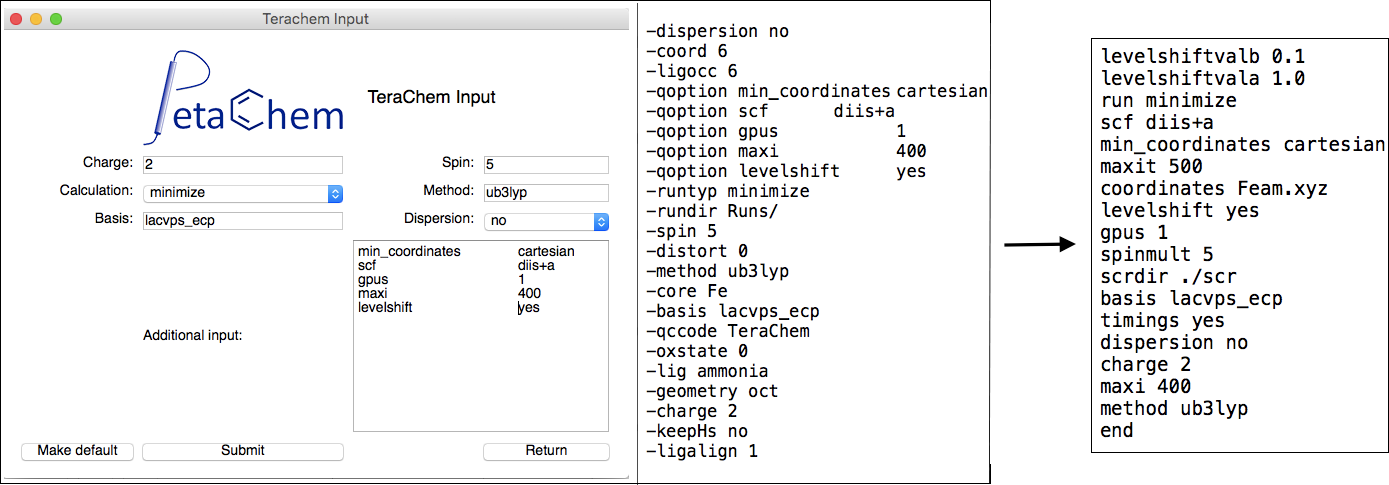
\includegraphics[width=\textwidth]{./Figures/fig10.png}
\caption{Parameters for generation of QC input files.}
\label{inp1}
\end{figure}

The final input file produced by the program is shown in Figure \ref{inp1}. Note that the program supports multiple methods, spins and charges, so if the user specifies for example for the method \texttt{ub3lyp,pbe} and charges \texttt{2,3} molSimplify will create 4 different folders each with one method and one charge.

Furthermore, in order to avoid entering similar input parameters every time the user wants to generate input files, there is a \texttt{Make default} option on the GUI that will overwrite the default options with the current ones.


\subsection{Jobscript generation}

In addition to the input files, molSimplify can generate jobscripts for supercomputer queues. Tow supercomputer queuing systems are currently supported, SGE and SLURM. 

On the GUI the user can enable the jobscript generation, select the target queuing system and bring up the corresponding window. Standard options here include the job name base (keyword \texttt{-jname}), queue name  (keyword \texttt{-queue}), wall time requested  (keyword \texttt{-wtime}), memory  (keyword \texttt{-memory}), number of cpu or gpus  (keywords \texttt{-cpus,-gpus}) and the modules to be loaded  (keyword \texttt{modules}). Additional options can be specified in the \texttt{Options} field or using the keyword \texttt{-joption} in the input file. Also extra commands for the jobscript can be specified in the corresponding field \texttt{Commands} or using the \texttt{jcommand} keyword in the input file.

\begin{figure}[htb!]
\centering
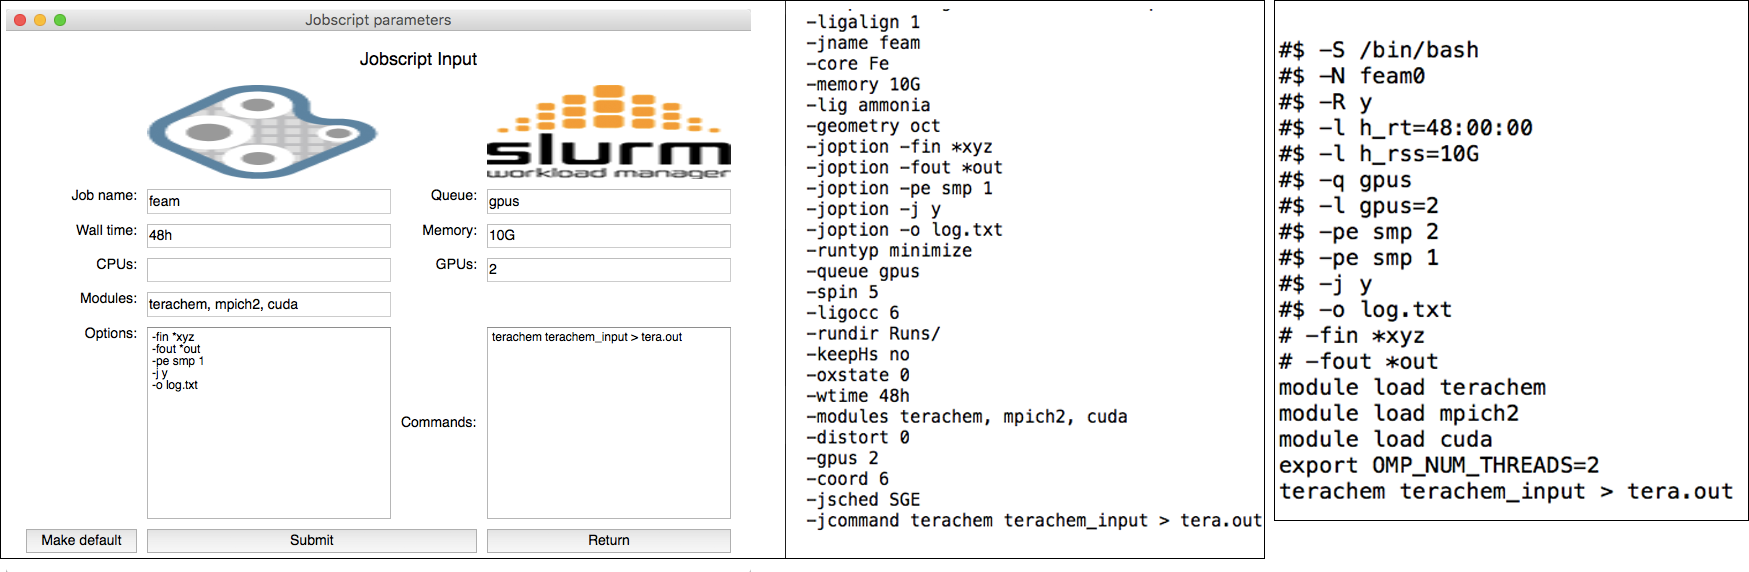
\includegraphics[width=\textwidth]{./Figures/fig11.png}
\caption{Parameters for jobscript generation.}
\label{job1}
\end{figure}

Figure \ref{job1} shows the jobscript generated using the specified input on the GUI. Furthermore, in order to avoid entering similar input parameters every time the user wants to generate jobscripts, there is a \texttt{Make default} option on the GUI that will overwrite the default options with the current ones.

\section{Similarity search \& screening}

An additional module, complementary to the structure generation is the similarity search and screening of chemical databases. The program is able to search for molecules in chemical databases and use the results to build sets of structures. 

The similarity search can be enabled by selecting the \texttt{Search DB} option on the GUI and bringing up the Chemical Database Search window (Figure \ref{db1}). 

\begin{figure}[htb!]
\centering
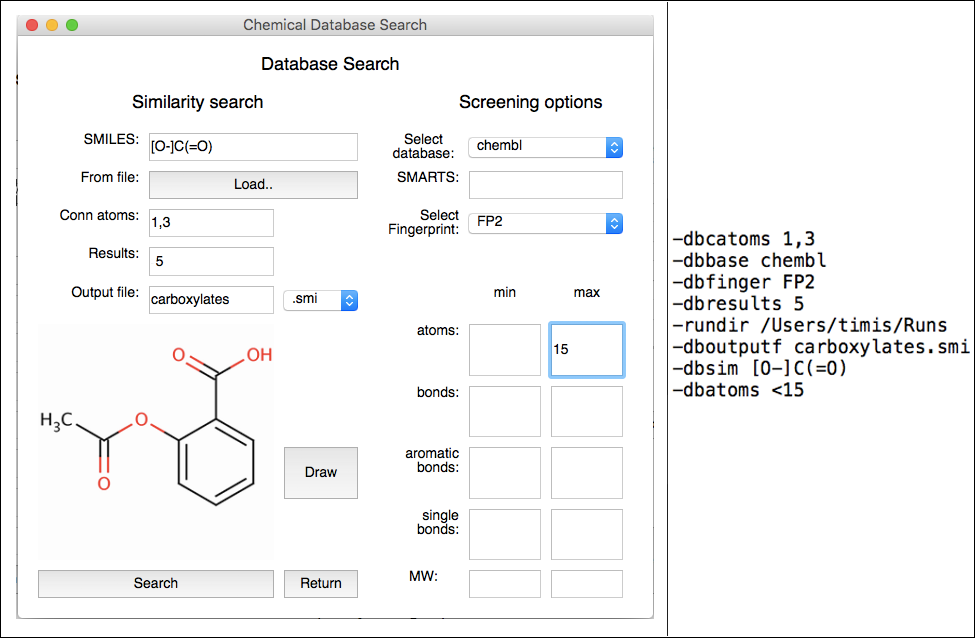
\includegraphics[width=\textwidth]{./Figures/fig14a.png}
\caption{Input parameters for Chemical Database search.}
\label{db1}
\end{figure}

In this example, we will use the database search to look for carboxylates. To search for similar structures in the \texttt{SMILES} field of the GUI (keyword \texttt{-dbsim}) we specify the string for a carboxylate structure. Alternatively, we can search for similar structures using an input file (xyz, mol or smi) and loading the file. Because, we want to use the results from the screening for structure generation, we specify the connection atoms on the carboxylate SMILES string (1 and 3 corresponding to the two oxygens in this case) and the program will automatically calculate the connection atoms on the screening results. The input file keyword for the connection atoms is \texttt{-dbcatoms}. The we select the number of carboxylate molecules that we want (keyword \texttt{-dbresults}) and the output file name (keyword \texttt{-dboutputf}). In addition or simultaneously to similarity search, we can directly screen the database for specific structures using a SMARTS string (keyword \texttt{-dbsmarts}). For example, if someone wants to find structures similar to carboxylates that contain at leaste on double carbon carbon bond, the SMARTS string \texttt{C=C} should be specified in the corresponding field.

 In any case we need to select the database we will use (keyword \texttt{-dbbase}). For screening, we can select various parameters, first the fingerprint used in the similarity search (keyword \texttt{-dbfinger}) and then options for the minimum and maximum number of atoms (keyword \texttt{-dbatoms}), the minimum and maximum number of bonds (keyword \texttt{-dbbonds}), the minimum and maximum number of aromatic bonds (keyword \texttt{-dbarbonds}), the minimum and maximum number of single bonds (keyword \texttt{-dbsbonds}) or the minimum and maximum molecular weight (keyword \texttt{-dbmw}).

\begin{figure}[htb!]
\centering
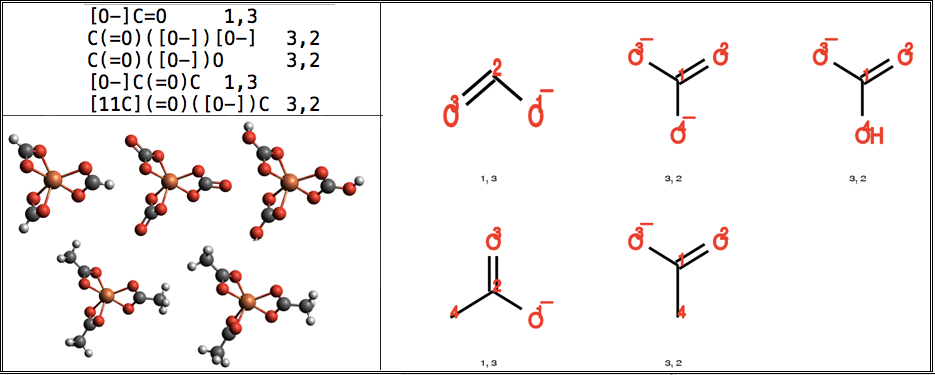
\includegraphics[width=\textwidth]{./Figures/fig14b.png}
\caption{Results of Database search and structure generation using those results.}
\label{db2}
\end{figure}

Once the similarity search is concluded, an output file with the SMILES strings of the corresponding results will be generated under the running directory (Figure \ref{db2}, top left). Note that because complexes are filtered to avoid salts and duplicates, the final number of structures might be smaller than the one specified in the beginning. The results of the search can be visualized using the \texttt{Draw} option (Figure \ref{db2}, right). Furthermore, the resulting SMILES file can be used as an input for structure generation. If the user specifies that file as a ligand, the program will loop over all results and generate one structure for each entry (Figure \ref{db2}, bottom left).


\section{Post processing}

An additional feature of molSimplify is post processing of Quantum Chemistry output. The parsing and processing of the output files is done using custom routines embedded in the program and using the external software Multiwfn. 

To enable the post processing routines, the corresponding option must be selected from the GUI and it will bring up the setup window (keyword \texttt{-postp}). The available options for post-processing start by selecting the directory of the output files (keyword \texttt{-postdir}) and the QC code that was used to run the jobs (keyword \texttt{-postqc}). Note that your output files should have a .out extension in order for the program to be able to find it. 

\begin{figure}[htb!]
\centering
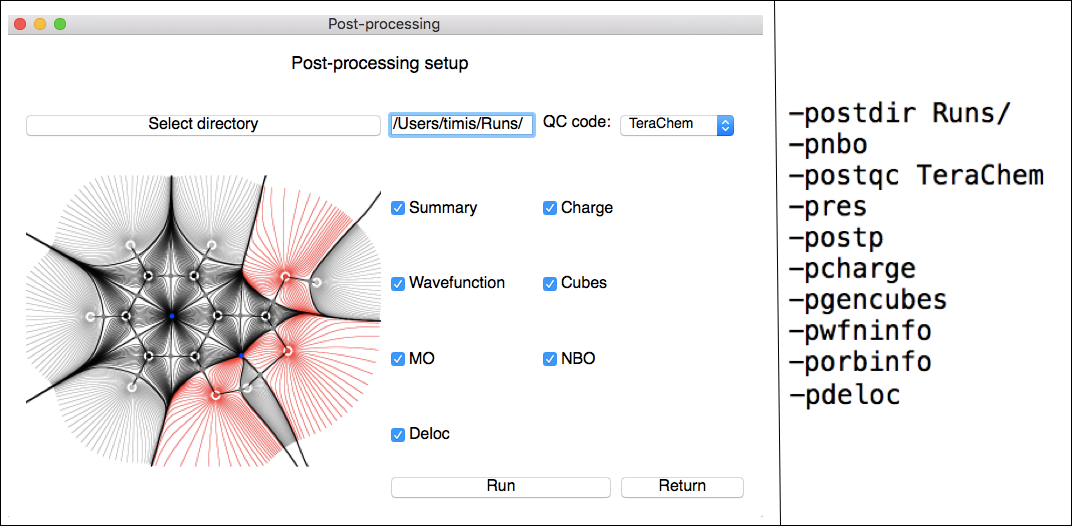
\includegraphics[width=\textwidth]{./Figures/fig15.png}
\caption{Input options for post-processing.}
\label{post0}
\end{figure}

The parsing and processing options include a summary of the results (keyword \texttt{-pres}) that contains information about the jobs such as energies, charges, runtime or spin state. Next, charges can be calculated (keyword \texttt{-pcharge}) using Multiwfn (currently supporting VDD, Mulliken and Hirshfeld charges). The wavefunction can be directly processed to get information such as the average electron distance, the variance of the electron positions, the HELP value or the average ELF (keyword \texttt{-pwfninfo}). The program is able to generate cube files for further processing (keyword \texttt{-pgencubes}) for the density, the spin density, $\alpha$ and $\beta$ electron densities and the ELF. Information about the molecular orbitals (HOMO, LUMO, Fermi energy, d-band center) can be generated as well (keyword \texttt{-porbinfo}) as well as parsing of NBO data (keyword \texttt{-pnbo}). Finally the localization and delocalization indices of the metal can be calculated as well using QTAIM (keyword \texttt{-pdeloc}).

\begin{figure}[htb!]
\centering
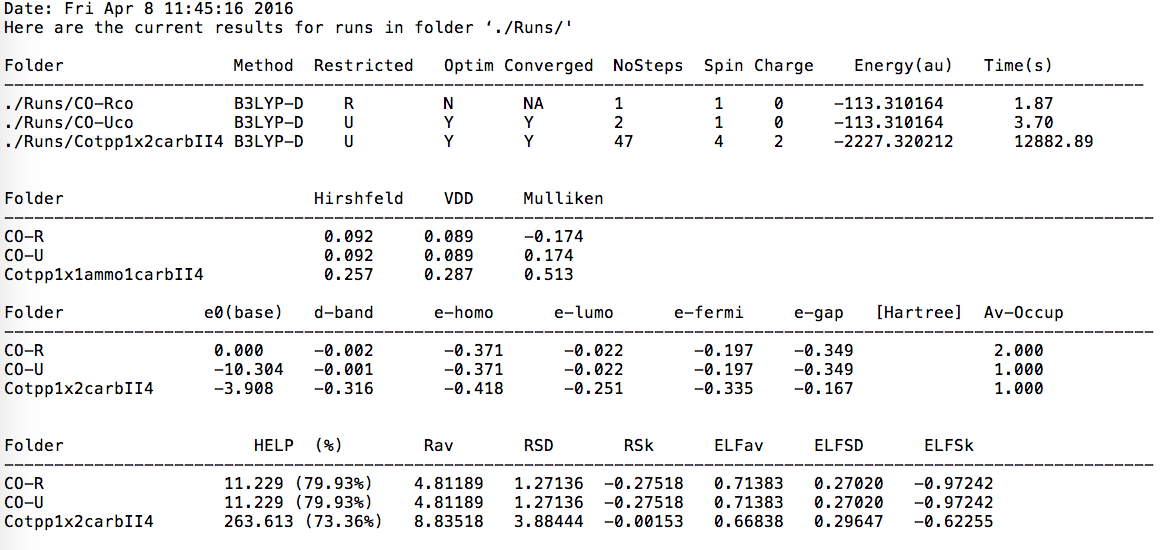
\includegraphics[width=\textwidth]{./Figures/fig16.png}
\caption{Example output summary files from the post processing module.}
\label{post1}
\end{figure}

Various files are generated during the post-processing, each placed in a folder corresponding to the property being calculated. The summary of the results is placed on the top jobs directory. An example of some summary files are included in Figure \ref{post1}.

\section{Extras}

\subsection{Updating the database}

The local database can be updated by adding or removing molecules. The window for updating the database is enabled using the \texttt{Add to local DB} button on the GUI (Figure \ref{ldb}).


\begin{figure}[htb!]
\centering
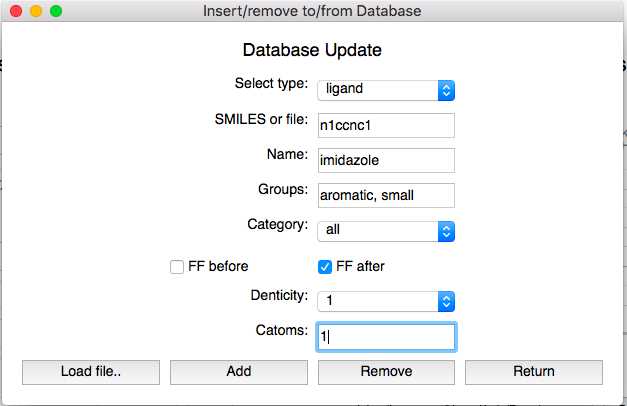
\includegraphics[width=0.5\textwidth]{./Figures/fig17.png}
\caption{Window for updating the local molecule database.}
\label{ldb}
\end{figure}

Updating the database starts by selecting what type of structure you want to add/remove (ligand, core or binding/extra molecule). Then the SMILES string of the molecule or the path to an xyz/mol file is specified. The \texttt{Load file} feature can be used as well to load a molecular file. Then a name is specified for the new molecule. If the molecule is a ligand the corresponding groups and categories are specified and then the denticity and the connection atoms of the ligand. Also the options for force field optimization can be specified here. If a force field optimization option is deselected, the ligand will be blacklisted from the optimization and will not be included in any optimization when building structures. 

A structure can be removed by specifying its name and then clicking the remove button. If someone wants to manually add/edit molecules, these are located in the installation directory as specified in the \texttt{$\sim$/.molSimplify} file under Cores, Ligands and Bind.

\subsection{Add geometry}

New coordination geometries can be added using the corresponding interface on the GUI. The window for updating the geometries is enabled using the \texttt{Add geometry} button on the GUI.

\begin{figure}[htb!]
\centering
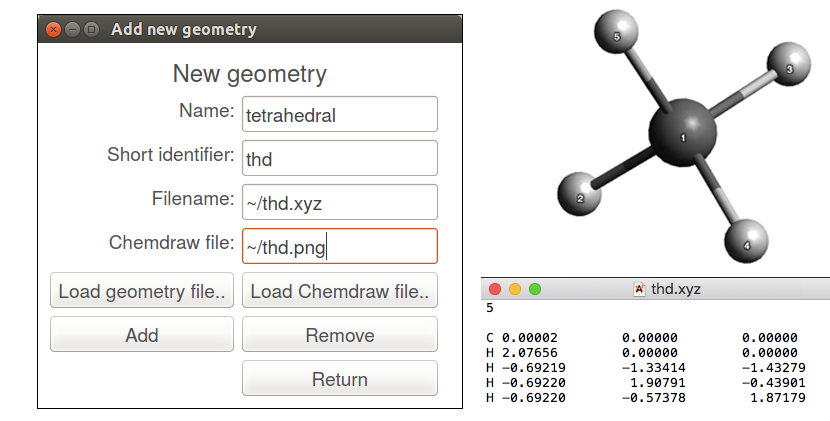
\includegraphics[width=0.75\textwidth]{./Figures/fig18.png}
\caption{Window for updating the coordination geometries.}
\label{lg}
\end{figure}

In order to add a new coordination geometry, the user needs to specify a name for the geometry and a short identifier (max 4 letters). Then an xyz file should be specified that will define the geometry. This file should include the minimum number of atoms that completely define the geometry with the metal center being the 1st atom in the file. An example is included in Figure \ref{lg} where a tetrahedral geometry is added. Finally a png file that shows a 2D Chemdraw of the geometry along with the atomic labels can be optionally included (see the default geometries on the GUI for examples).

To manually add/edit geometries these are located in the installation directory as specified in the \texttt{$\sim$/.molSimplify} file under Data and the png files under icons/geoms.

\section{Command line options}

A full list of the command line options used in the input files or directly as additional arguments is included here: \\


\centering
\small
\begin{tabular}{|l|l|l|}
\hline
\textit{\textbf{Keyword}} & \textit{\textbf{Description}} & \textit{\textbf{Default value}} \\
\hline
%% ----------------------------------------------------------------------------------------------- %%
\multicolumn{3}{|c|}{\Large \textbf{General parameters}}\\ \hline
\texttt{-help} & show help message & - \\
\texttt{-i} & input file & - \\
\texttt{-rundir} & directory for jobs & /home/user/Runs \\
\texttt{-jobdir} & directory name for this specific job (relative to -rundir)  & (based on complex) \\
\texttt{-name} & name for this specific complex (relative to -jobdir)  & (based on complex)\footnotemark\\
\texttt{-suff} & suffix for jobs folder & - \\
\texttt{-genall} & generate complex both with and without FF opt. & \texttt{False} \\
\hline
\end{tabular}
\footnotetext{In the general case, output will be found under rundir/jobdir/name.xyx}
\begin{tabular}{|l|l|l|}
\hline
\multicolumn{3}{|c|}{\Large \textbf{Structure generation parameters}}\\ \hline   
\texttt{-core} & core structure  & - \\
\texttt{-ccatoms} & custom core connection atom(s) indices & - \\
\texttt{-replig} & flag for modify/replace feature & \texttt{False} \\
\texttt{-geometry} & coordination geometry & \texttt{oct} (octahedral) \\
\texttt{-coord} & coordination number & \texttt{6} \\
\texttt{-lig} & ligand structure name, SMILES  or file path& - \\
\texttt{-ligocc} &  frequency of corresponding ligands & \texttt{1} \\
\texttt{-keepHs} & do not remove Hydrogens from ligand & \texttt{False} \\
\texttt{-smicat} & custom ligand connection atom(s) indices & - \\
\texttt{-sminame} & custom ligand name  & - \\
\texttt{-ligloc} & force location of ligands on the template & \texttt{False} \\
\texttt{-ligalign} & smart alignment of ligands  & \texttt{True} \\
\texttt{-MLbonds} & custom M-L bond length for ligand (A)  & \texttt{database value} \\
\texttt{-rgen} & number of random generated molecules & \texttt{1} \\
\texttt{-lignum} & number of different ligands in random generation & - \\
\texttt{-liggrp} & ligand group for random generation & \texttt{all} \\
\texttt{-ligctg} & ligand category for random generation & \texttt{all} \\
\texttt{-rkHs} & keep Hydrogens for random generation & \texttt{False} \\
\texttt{-ff} & select force field for FF optimization & \texttt{MMFF94} \\
\texttt{-ffoption} & select when to perform FF optimization & \texttt{Before \& Afte}r \\
\texttt{-distort} & randomly distort backbone by x\% & \texttt{0\%} \\
\texttt{-langles} & custom angles (polar, azimuthal) for ligand & \texttt{0/0} \\
\hline
\end{tabular}

%% ----------------------------------------------------------------------------------------------- %%
\begin{tabular}{|l|l|l|}
\hline
\multicolumn{3}{|c|}{\Large \textbf{Extra molecules parameters}}\\ \hline
\texttt{-bind} & extra molecule name, SMILES or file & \texttt{False} \\
\texttt{-bcharge} & binding species charge & \texttt{0} \\
\texttt{-bph} & azimuthal angle phi for binding species & \texttt{random} \\
\texttt{-bref} & reference atoms for placement of extra molecules &  \texttt{COM}  \\
\texttt{-bsep} & flag for separating extra molecule in input or xyz file & False \\
\texttt{-btheta} & polar angle theta for binding species & \texttt{random} \\
\texttt{-place} & azimuthal angle for binding species relative to core & \texttt{random} \\
\texttt{-bindnum} & number of binding species copies for random placement & \texttt{1} \\
\texttt{-nambsmi} & name of custom extra molecule & - \\
\texttt{-maxd} & maximum distance for molecule placement (A) & \texttt{0.0} \\
\texttt{-mind} & minimum distance for molecule placement (A) & \texttt{0.0} \\
\texttt{-oxstate} &  oxidation state of the metal & \texttt{0} \\
\hline
\end{tabular}

%%---------------------------------------------------------------------------------------------- %%
\begin{tabular}{|l|l|l|}
\hline
\multicolumn{3}{|c|}{\Large \textbf{Jobscript parameters}}\\ \hline                        
\texttt{-jsched} & job scheduling system & \texttt{SGE} \\
\texttt{-jname} & jobs main identifier & - \\
\texttt{-memory} & memory reserved per thread for job file in G & \texttt{2G} \\
\texttt{-wtime} & wall time requested in hours for queueing system  & \texttt{168h} \\
\texttt{-queue} & queue name & \texttt{gpus} \\
\texttt{-gpus} & number of GPUS & \texttt{1} \\
\texttt{-cpus} & number of CPUs  & \texttt{1} \\
\texttt{-modules} &  modules to be loaded for the calculation & - \\
\texttt{-joption} & additional options for jobscript & - \\
\texttt{-jcommand} & additional commands for jobscript & - \\
\hline
\end{tabular}
%%
\begin{tabular}{|l|c|c|}
\hline
\multicolumn{3}{|c|}{\Large\textbf{Post-processing parameters}}\\ \hline
\texttt{-postp} & post process results & - \\
\texttt{-postqc} & quantum chemistry code used & \texttt{TeraChem} \\
\texttt{-postdir} & directory with results & \texttt{/home/user/Runs} \\
\texttt{-pres} & generate calculations summary & \texttt{False} \\
\texttt{-pdeninfo} &  calculate average properties for electron density & \texttt{False} \\
\texttt{-pcharge} &   calculate charges & \texttt{False} \\
\texttt{-pgencubes} & generate cubefiles & \texttt{False} \\
\texttt{-pwfninfo} & get information about wavefunction & \texttt{False} \\
\texttt{-pdeloc} &     get delocalization and localization indices & \texttt{False} \\
\texttt{-porbinfo} & get information about MO & \texttt{False} \\
\texttt{-pnbo} & post process nbo analysis & \texttt{False} \\
\hline
\end{tabular}


 ----------------------------------------------------------------------------------------------- %%
\begin{tabular}{|l|l|l|}
\hline
 \multicolumn{3}{|c|}{\Large \textbf{Quantum chemistry input}}\\ \hline 
\texttt{-qccode} & quantum chemistry code & \texttt{TeraChem} \\
\texttt{-charge} & charge for system & \texttt{0} \\
\texttt{-calccharge} & flag to calculate charge & \texttt{False} \\
\texttt{-spin} & spin multiplicity for system  & \texttt{1} \\
\texttt{-runtyp} & run type  & \texttt{optimize} \\
\texttt{-method} & electronic structure method & \texttt{ub3lyp} \\
\texttt{-basis} & basis for terachem or qchem job  & \texttt{lacvp*} \\
\texttt{-dispersion} & dispersion forces & \texttt{False} \\
\texttt{-qoption} & extra arguments for TeraChem in syntax& - \\
\texttt{-exchange} & exchange in qchem job  & \texttt{b3lyp} \\
\texttt{-correlation} & correlation in qchem job  & \texttt{none} \\
\texttt{-remoption} & extra arguments for qchem \$rem block& - \\
\texttt{-unrestricted} & unrestricted calculation & True \\
\texttt{-gbasis} & GBASIS option in GAMESS & \texttt{6} \\
\texttt{-ngauss} & NGAUSS option in GAMESS  & \texttt{N31} \\
\texttt{-npfunc} & NPFUNC option for diffuse functions in GAMESS  & - \\
\texttt{-ndfunc} & NDFUNC option for diffuse functions in GAMESS  & - \\
\texttt{-sysoption} & extra arguments for \$SYSTEM GAMESS block & - \\
\texttt{-ctrloption} & extra arguments for \$CONTRL GAMESS block & - \\
\texttt{-scfoption} & extra arguments for \$SCF GAMESS block & - \\
\texttt{-statoption} & extra arguments for \$STATPT GAMESS block & - \\
\hline
\end{tabular}
%% -
%% ----------------------------------------------------------------------------------------------- %%
\begin{tabular}{|l|l|l|}
\hline
\multicolumn{3}{|c|}{\Large \textbf{Database search input}}\\ \hline                        
\texttt{-dbsim} & SMILES/ligand/file for similarity search & - \\
\texttt{-dbcatoms} & connection atoms for similarity search & - \\
\texttt{-dbresults} & how many results for similary search or screening & - \\
\texttt{-dboutputf} & output file for search results & \texttt{simres.smi} \\
\texttt{-dbbase} & database for search & - \\
\texttt{-dbsmarts} & SMARTS string for screening & - \\
\texttt{-dbfinger} & fingerprint for similarity search & - \\
\texttt{-dbatoms} & number of atoms to be used in screening & - \\
\texttt{-dbbonds} & number of bonds to be used in screening & - \\
\texttt{-dbarbonds} & number of aromatic bonds to be used in screening & - \\
\texttt{-dbsbonds} & number of single bonds to be used in screening & - \\
\texttt{-dbmw} & molecular weight to be used in screening & - \\
\hline
\end{tabular}
%% ----------------------------------------------------------------------------------------------- 

\bibliographystyle{plain}
\bibliography{Bib/refs}



\end{document}